\documentclass[../masters.tex]{subfiles}

\begin{document}
\graphicspath{{./imgs/}{../imgs/}} %look for images

\section{Linear Models}
In this section we consider probabilistic graphical models of the form shown in Figure \ref{fig_linmod}. Firstly we investigate a model where the states ($X$) and observations ($Y$) are discrete. Models of this form are classically called Hidden Markov Models (HMMs). Secondly we generalise the model to include continuous states and observations. Models of this form are called Latent Linear Dynamical Systems (the famous Kalman Filter model falls into this category). We assume in both cases that the states are hidden but the observations are visible.
\begin{figure}[H] 
\centering
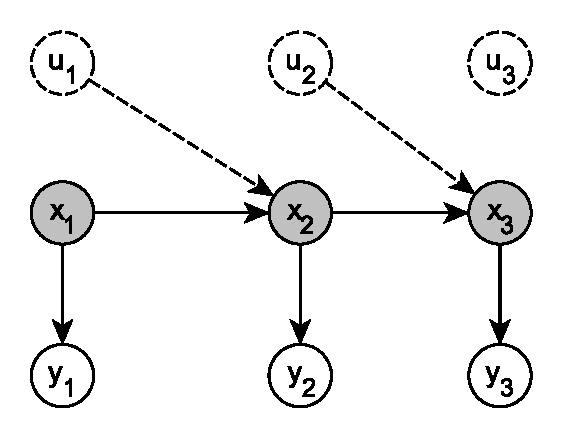
\includegraphics[scale=1.0]{linear_model.pdf}
\caption{Linear Graphical Model}
\label{fig_linmod}
\end{figure}

\subsection{Discrete Models}


\subsection{Continuous Models}

\end{document}